% !TeX program = pdflatex
% !TeX root = DiracSimplify.tex

\documentclass[../FeynCalcManual.tex]{subfiles}
\begin{document}
\hypertarget{diracsimplify}{
\section{DiracSimplify}\label{diracsimplify}\index{DiracSimplify}}

\texttt{DiracSimplify[\allowbreak{}exp]} simplifies products of Dirac
matrices in \texttt{exp} and expands noncommutative products. The
simplifications are done by applying \texttt{Contract},
\texttt{DiracEquation}, \texttt{DiracTrick}, \texttt{SpinorChainTrick}
and \texttt{SirlinSimplify}. All \(\gamma^5\), \(\gamma^6\) and
\(\gamma^7\) are moved to the right. The order of the other Dirac
matrices is not changed, unless the option DiracOrder is set to
\texttt{True}.

\subsection{See also}

\hyperlink{toc}{Overview}, \hyperlink{contract}{Contract},
\hyperlink{diracequation}{DiracEquation},
\hyperlink{diracsigmaexplicit}{DiracSigmaExplicit},
\hyperlink{diracsubstitute5}{DiracSubstitute5},
\hyperlink{diracsubstitute67}{DiracSubstitute67},
\hyperlink{diracgamma}{DiracGamma},
\hyperlink{diracgammaexpand}{DiracGammaExpand},
\hyperlink{diracorder}{DiracOrder}, \hyperlink{diractrace}{DiracTrace},
\hyperlink{diractraceevaluate}{DiracTraceEvaluate},
\hyperlink{diractrick}{DiracTrick},
\hyperlink{fcdiracisolate}{FCDiracIsolate},
\hyperlink{sirlinsimplify}{SirlinSimplify},
\hyperlink{spinorchaintrick}{SpinorChainTrick},
\hyperlink{spinorchainevaluate}{SpinorChainEvaluate},
\hyperlink{todiracgamma67}{ToDiracGamma67}.

\subsection{Examples}

Simplify a 4-dimensional Dirac matrix chain with a dummy Lorentz index

\begin{Shaded}
\begin{Highlighting}[]
\NormalTok{GA}\OperatorTok{[}\SpecialCharTok{\textbackslash{}}\OperatorTok{[}\NormalTok{Mu}\OperatorTok{],} \SpecialCharTok{\textbackslash{}}\OperatorTok{[}\NormalTok{Nu}\OperatorTok{],} \SpecialCharTok{\textbackslash{}}\OperatorTok{[}\NormalTok{Mu}\OperatorTok{]]} 
 
\NormalTok{DiracSimplify}\OperatorTok{[}\SpecialCharTok{\%}\OperatorTok{]}
\end{Highlighting}
\end{Shaded}

\begin{dmath*}\breakingcomma
\bar{\gamma }^{\mu }.\bar{\gamma }^{\nu }.\bar{\gamma }^{\mu }
\end{dmath*}

\begin{dmath*}\breakingcomma
-2 \bar{\gamma }^{\nu }
\end{dmath*}

Another common simplification concerns Dirac matrices contracted to the
same \(4\)-vector

\begin{Shaded}
\begin{Highlighting}[]
\NormalTok{GS}\OperatorTok{[}\FunctionTok{p}\OperatorTok{]}\NormalTok{ . GS}\OperatorTok{[}\FunctionTok{p}\OperatorTok{]} 
 
\NormalTok{DiracSimplify}\OperatorTok{[}\SpecialCharTok{\%}\OperatorTok{]}
\end{Highlighting}
\end{Shaded}

\begin{dmath*}\breakingcomma
\left(\bar{\gamma }\cdot \overline{p}\right).\left(\bar{\gamma }\cdot \overline{p}\right)
\end{dmath*}

\begin{dmath*}\breakingcomma
\overline{p}^2
\end{dmath*}

Unlike \texttt{DiracTrick}, \texttt{DiracSimplify} also carries out
noncommutative expansions

\begin{Shaded}
\begin{Highlighting}[]
\NormalTok{GS}\OperatorTok{[}\FunctionTok{a} \SpecialCharTok{+} \FunctionTok{b}\OperatorTok{]}\NormalTok{ . GS}\OperatorTok{[}\FunctionTok{p}\OperatorTok{]}\NormalTok{ . GS}\OperatorTok{[}\FunctionTok{c} \SpecialCharTok{+} \FunctionTok{d}\OperatorTok{]}\NormalTok{ . GS}\OperatorTok{[}\FunctionTok{p}\OperatorTok{]} 
 
\NormalTok{DiracSimplify}\OperatorTok{[}\SpecialCharTok{\%}\OperatorTok{]}
\end{Highlighting}
\end{Shaded}

\begin{dmath*}\breakingcomma
\left(\bar{\gamma }\cdot \left(\overline{a}+\overline{b}\right)\right).\left(\bar{\gamma }\cdot \overline{p}\right).\left(\bar{\gamma }\cdot \left(\overline{c}+\overline{d}\right)\right).\left(\bar{\gamma }\cdot \overline{p}\right)
\end{dmath*}

\begin{dmath*}\breakingcomma
2 \left(\overline{c}\cdot \overline{p}\right) \left(\bar{\gamma }\cdot \overline{a}\right).\left(\bar{\gamma }\cdot \overline{p}\right)-\overline{p}^2 \left(\bar{\gamma }\cdot \overline{a}\right).\left(\bar{\gamma }\cdot \overline{c}\right)+2 \left(\overline{d}\cdot \overline{p}\right) \left(\bar{\gamma }\cdot \overline{a}\right).\left(\bar{\gamma }\cdot \overline{p}\right)-\overline{p}^2 \left(\bar{\gamma }\cdot \overline{a}\right).\left(\bar{\gamma }\cdot \overline{d}\right)+2 \left(\overline{c}\cdot \overline{p}\right) \left(\bar{\gamma }\cdot \overline{b}\right).\left(\bar{\gamma }\cdot \overline{p}\right)-\overline{p}^2 \left(\bar{\gamma }\cdot \overline{b}\right).\left(\bar{\gamma }\cdot \overline{c}\right)+2 \left(\overline{d}\cdot \overline{p}\right) \left(\bar{\gamma }\cdot \overline{b}\right).\left(\bar{\gamma }\cdot \overline{p}\right)-\overline{p}^2 \left(\bar{\gamma }\cdot \overline{b}\right).\left(\bar{\gamma }\cdot \overline{d}\right)
\end{dmath*}

\begin{Shaded}
\begin{Highlighting}[]
\NormalTok{DiracTrick}\OperatorTok{[}\NormalTok{GS}\OperatorTok{[}\FunctionTok{a} \SpecialCharTok{+} \FunctionTok{b}\OperatorTok{]}\NormalTok{ . GS}\OperatorTok{[}\FunctionTok{p}\OperatorTok{]}\NormalTok{ . GS}\OperatorTok{[}\FunctionTok{c} \SpecialCharTok{+} \FunctionTok{d}\OperatorTok{]}\NormalTok{ . GS}\OperatorTok{[}\FunctionTok{p}\OperatorTok{]]}
\end{Highlighting}
\end{Shaded}

\begin{dmath*}\breakingcomma
2 \left(\bar{\gamma }\cdot \left(\overline{a}+\overline{b}\right)\right).\left(\bar{\gamma }\cdot \overline{p}\right) \left((\overline{c}+\overline{d})\cdot \overline{p}\right)-\overline{p}^2 \left(\bar{\gamma }\cdot \left(\overline{a}+\overline{b}\right)\right).\left(\bar{\gamma }\cdot \left(\overline{c}+\overline{d}\right)\right)
\end{dmath*}

Some of those expansions can be inhibited via the option
\texttt{Expanding}.

\begin{Shaded}
\begin{Highlighting}[]
\NormalTok{DiracSimplify}\OperatorTok{[}\NormalTok{GS}\OperatorTok{[}\FunctionTok{a} \SpecialCharTok{+} \FunctionTok{b}\OperatorTok{]}\NormalTok{ . GS}\OperatorTok{[}\FunctionTok{p}\OperatorTok{]}\NormalTok{ . GS}\OperatorTok{[}\FunctionTok{c} \SpecialCharTok{+} \FunctionTok{d}\OperatorTok{]}\NormalTok{ . GS}\OperatorTok{[}\FunctionTok{p}\OperatorTok{],}\NormalTok{ Expanding }\OtherTok{{-}\textgreater{}} \ConstantTok{False}\OperatorTok{]}
\end{Highlighting}
\end{Shaded}

\begin{dmath*}\breakingcomma
-\overline{p}^2 \left(\bar{\gamma }\cdot \overline{a}+\bar{\gamma }\cdot \overline{b}\right).\left(\bar{\gamma }\cdot \overline{c}+\bar{\gamma }\cdot \overline{d}\right)+2 \left(\overline{c}\cdot \overline{p}\right) \left(\bar{\gamma }\cdot \overline{a}+\bar{\gamma }\cdot \overline{b}\right).\left(\bar{\gamma }\cdot \overline{p}\right)+2 \left(\overline{d}\cdot \overline{p}\right) \left(\bar{\gamma }\cdot \overline{a}+\bar{\gamma }\cdot \overline{b}\right).\left(\bar{\gamma }\cdot \overline{p}\right)
\end{dmath*}

The matrix chain may also live in \(D\) dimensions

\begin{Shaded}
\begin{Highlighting}[]
\NormalTok{GAD}\OperatorTok{[}\SpecialCharTok{\textbackslash{}}\OperatorTok{[}\NormalTok{Mu}\OperatorTok{],} \SpecialCharTok{\textbackslash{}}\OperatorTok{[}\NormalTok{Nu}\OperatorTok{],} \SpecialCharTok{\textbackslash{}}\OperatorTok{[}\NormalTok{Mu}\OperatorTok{]]} 
 
\NormalTok{DiracSimplify}\OperatorTok{[}\SpecialCharTok{\%}\OperatorTok{]}
\end{Highlighting}
\end{Shaded}

\begin{dmath*}\breakingcomma
\gamma ^{\mu }.\gamma ^{\nu }.\gamma ^{\mu }
\end{dmath*}

\begin{dmath*}\breakingcomma
2 \gamma ^{\nu }-D \gamma ^{\nu }
\end{dmath*}

\begin{Shaded}
\begin{Highlighting}[]
\NormalTok{GSD}\OperatorTok{[}\FunctionTok{p}\OperatorTok{]}\NormalTok{ . GAD}\OperatorTok{[}\SpecialCharTok{\textbackslash{}}\OperatorTok{[}\NormalTok{Alpha}\OperatorTok{],} \SpecialCharTok{\textbackslash{}}\OperatorTok{[}\FunctionTok{Beta}\OperatorTok{]]}\NormalTok{ . GSD}\OperatorTok{[}\FunctionTok{p}\OperatorTok{]} 
 
\NormalTok{DiracSimplify}\OperatorTok{[}\SpecialCharTok{\%}\OperatorTok{]}
\end{Highlighting}
\end{Shaded}

\begin{dmath*}\breakingcomma
(\gamma \cdot p).\gamma ^{\alpha }.\gamma ^{\beta }.(\gamma \cdot p)
\end{dmath*}

\begin{dmath*}\breakingcomma
p^2 \gamma ^{\alpha }.\gamma ^{\beta }+2 p^{\alpha } \gamma ^{\beta }.(\gamma \cdot p)-2 p^{\beta } \gamma ^{\alpha }.(\gamma \cdot p)
\end{dmath*}

\begin{Shaded}
\begin{Highlighting}[]
\NormalTok{GAD @@ }\FunctionTok{Join}\OperatorTok{[\{}\SpecialCharTok{\textbackslash{}}\OperatorTok{[}\NormalTok{Mu}\OperatorTok{]\},} \FunctionTok{Table}\OperatorTok{[}\FunctionTok{Subscript}\OperatorTok{[}\SpecialCharTok{\textbackslash{}}\OperatorTok{[}\NormalTok{Nu}\OperatorTok{],} \FunctionTok{i}\OperatorTok{],} \OperatorTok{\{}\FunctionTok{i}\OperatorTok{,} \DecValTok{6}\OperatorTok{\}],} \OperatorTok{\{}\SpecialCharTok{\textbackslash{}}\OperatorTok{[}\NormalTok{Mu}\OperatorTok{]\}]} 
 
\NormalTok{DiracSimplify}\OperatorTok{[}\SpecialCharTok{\%}\OperatorTok{]}
\end{Highlighting}
\end{Shaded}

\begin{dmath*}\breakingcomma
\gamma ^{\mu }.\gamma ^{\nu _1}.\gamma ^{\nu _2}.\gamma ^{\nu _3}.\gamma ^{\nu _4}.\gamma ^{\nu _5}.\gamma ^{\nu _6}.\gamma ^{\mu }
\end{dmath*}

\begin{dmath*}\breakingcomma
-12 \gamma ^{\nu _1}.\gamma ^{\nu _2}.\gamma ^{\nu _3}.\gamma ^{\nu _4}.\gamma ^{\nu _5}.\gamma ^{\nu _6}+D \gamma ^{\nu _1}.\gamma ^{\nu _2}.\gamma ^{\nu _3}.\gamma ^{\nu _4}.\gamma ^{\nu _5}.\gamma ^{\nu _6}+4 \gamma ^{\nu _3}.\gamma ^{\nu _4}.\gamma ^{\nu _5}.\gamma ^{\nu _6} g^{\nu _1\nu _2}-4 \gamma ^{\nu _2}.\gamma ^{\nu _4}.\gamma ^{\nu _5}.\gamma ^{\nu _6} g^{\nu _1\nu _3}+4 \gamma ^{\nu _2}.\gamma ^{\nu _3}.\gamma ^{\nu _5}.\gamma ^{\nu _6} g^{\nu _1\nu _4}-4 \gamma ^{\nu _2}.\gamma ^{\nu _3}.\gamma ^{\nu _4}.\gamma ^{\nu _6} g^{\nu _1\nu _5}+4 \gamma ^{\nu _2}.\gamma ^{\nu _3}.\gamma ^{\nu _4}.\gamma ^{\nu _5} g^{\nu _1\nu _6}+4 \gamma ^{\nu _1}.\gamma ^{\nu _4}.\gamma ^{\nu _5}.\gamma ^{\nu _6} g^{\nu _2\nu _3}-4 \gamma ^{\nu _1}.\gamma ^{\nu _3}.\gamma ^{\nu _5}.\gamma ^{\nu _6} g^{\nu _2\nu _4}+4 \gamma ^{\nu _1}.\gamma ^{\nu _3}.\gamma ^{\nu _4}.\gamma ^{\nu _6} g^{\nu _2\nu _5}-4 \gamma ^{\nu _1}.\gamma ^{\nu _3}.\gamma ^{\nu _4}.\gamma ^{\nu _5} g^{\nu _2\nu _6}+4 \gamma ^{\nu _1}.\gamma ^{\nu _2}.\gamma ^{\nu _5}.\gamma ^{\nu _6} g^{\nu _3\nu _4}-4 \gamma ^{\nu _1}.\gamma ^{\nu _2}.\gamma ^{\nu _4}.\gamma ^{\nu _6} g^{\nu _3\nu _5}+4 \gamma ^{\nu _1}.\gamma ^{\nu _2}.\gamma ^{\nu _4}.\gamma ^{\nu _5} g^{\nu _3\nu _6}+4 \gamma ^{\nu _1}.\gamma ^{\nu _2}.\gamma ^{\nu _3}.\gamma ^{\nu _6} g^{\nu _4\nu _5}-4 \gamma ^{\nu _1}.\gamma ^{\nu _2}.\gamma ^{\nu _3}.\gamma ^{\nu _5} g^{\nu _4\nu _6}+4 \gamma ^{\nu _1}.\gamma ^{\nu _2}.\gamma ^{\nu _3}.\gamma ^{\nu _4} g^{\nu _5\nu _6}
\end{dmath*}

\begin{Shaded}
\begin{Highlighting}[]
\SpecialCharTok{{-}}\DecValTok{1}\SpecialCharTok{/}\DecValTok{2}\NormalTok{ GA}\OperatorTok{[}\DecValTok{5}\OperatorTok{]}\NormalTok{ . (GAD}\OperatorTok{[}\SpecialCharTok{\textbackslash{}}\OperatorTok{[}\NormalTok{Mu}\OperatorTok{]]}\NormalTok{ . GSD}\OperatorTok{[}\FunctionTok{v}\OperatorTok{]} \SpecialCharTok{{-}}\NormalTok{ FVD}\OperatorTok{[}\FunctionTok{v}\OperatorTok{,} \SpecialCharTok{\textbackslash{}}\OperatorTok{[}\NormalTok{Mu}\OperatorTok{]]}\NormalTok{) FVD}\OperatorTok{[}\FunctionTok{v}\OperatorTok{,} \SpecialCharTok{\textbackslash{}}\OperatorTok{[}\NormalTok{Mu}\OperatorTok{]]} 
 
\NormalTok{DiracSimplify}\OperatorTok{[}\SpecialCharTok{\%}\OperatorTok{]}
\end{Highlighting}
\end{Shaded}

\begin{dmath*}\breakingcomma
-\frac{1}{2} v^{\mu } \bar{\gamma }^5.\left(\gamma ^{\mu }.(\gamma \cdot v)-v^{\mu }\right)
\end{dmath*}

\begin{dmath*}\breakingcomma
0
\end{dmath*}

\(\gamma^5\) and the chirality projectors are always moved to the right

\begin{Shaded}
\begin{Highlighting}[]
\NormalTok{GA}\OperatorTok{[}\DecValTok{5}\OperatorTok{,} \SpecialCharTok{\textbackslash{}}\OperatorTok{[}\NormalTok{Mu}\OperatorTok{],} \SpecialCharTok{\textbackslash{}}\OperatorTok{[}\NormalTok{Nu}\OperatorTok{]]} 
 
\NormalTok{DiracSimplify}\OperatorTok{[}\SpecialCharTok{\%}\OperatorTok{]}
\end{Highlighting}
\end{Shaded}

\begin{dmath*}\breakingcomma
\bar{\gamma }^5.\bar{\gamma }^{\mu }.\bar{\gamma }^{\nu }
\end{dmath*}

\begin{dmath*}\breakingcomma
\bar{\gamma }^{\mu }.\bar{\gamma }^{\nu }.\bar{\gamma }^5
\end{dmath*}

\begin{Shaded}
\begin{Highlighting}[]
\NormalTok{GA}\OperatorTok{[}\DecValTok{6}\OperatorTok{]}\NormalTok{ . GS}\OperatorTok{[}\FunctionTok{p} \SpecialCharTok{+} \FunctionTok{q}\OperatorTok{]} 
 
\NormalTok{DiracSimplify}\OperatorTok{[}\SpecialCharTok{\%}\OperatorTok{]}
\end{Highlighting}
\end{Shaded}

\begin{dmath*}\breakingcomma
\bar{\gamma }^6.\left(\bar{\gamma }\cdot \left(\overline{p}+\overline{q}\right)\right)
\end{dmath*}

\begin{dmath*}\breakingcomma
\left(\bar{\gamma }\cdot \overline{p}\right).\bar{\gamma }^7+\left(\bar{\gamma }\cdot \overline{q}\right).\bar{\gamma }^7
\end{dmath*}

The properties of the chirality projectors are taken into account
without substituting explicit expressions for \(\gamma^6\) and
\(\gamma^7\).

\begin{Shaded}
\begin{Highlighting}[]
\NormalTok{GA}\OperatorTok{[}\SpecialCharTok{\textbackslash{}}\OperatorTok{[}\NormalTok{Mu}\OperatorTok{]]}\NormalTok{ . (c1 GA}\OperatorTok{[}\DecValTok{6}\OperatorTok{]} \SpecialCharTok{+}\NormalTok{ c2 GA}\OperatorTok{[}\DecValTok{7}\OperatorTok{]}\NormalTok{) . (GA}\OperatorTok{[}\FunctionTok{p}\OperatorTok{]} \SpecialCharTok{+} \FunctionTok{m}\NormalTok{) . (c3 GA}\OperatorTok{[}\DecValTok{6}\OperatorTok{]} \SpecialCharTok{+}\NormalTok{ c4 GA}\OperatorTok{[}\DecValTok{7}\OperatorTok{]}\NormalTok{) . GA}\OperatorTok{[}\SpecialCharTok{\textbackslash{}}\OperatorTok{[}\NormalTok{Mu}\OperatorTok{]]} 
 
\NormalTok{DiracSimplify}\OperatorTok{[}\SpecialCharTok{\%}\OperatorTok{]}
\end{Highlighting}
\end{Shaded}

\begin{dmath*}\breakingcomma
\bar{\gamma }^{\mu }.\left(\text{c1} \bar{\gamma }^6+\text{c2} \bar{\gamma }^7\right).\left(\bar{\gamma }^p+m\right).\left(\text{c3} \bar{\gamma }^6+\text{c4} \bar{\gamma }^7\right).\bar{\gamma }^{\mu }
\end{dmath*}

\begin{dmath*}\breakingcomma
4 \;\text{c1} \;\text{c3} m \bar{\gamma }^7-2 \;\text{c1} \;\text{c4} \bar{\gamma }^p.\bar{\gamma }^6-2 \;\text{c2} \;\text{c3} \bar{\gamma }^p.\bar{\gamma }^7+4 \;\text{c2} \;\text{c4} m \bar{\gamma }^6
\end{dmath*}

Moreover, \(\frac{1}{2} \left( 1 \pm \gamma^5 \right)\) is automatically
replaced by \(\gamma^{6/7}\).

\begin{Shaded}
\begin{Highlighting}[]
\NormalTok{(}\DecValTok{1}\SpecialCharTok{/}\DecValTok{2} \SpecialCharTok{{-}}\NormalTok{ GA}\OperatorTok{[}\DecValTok{5}\OperatorTok{]}\SpecialCharTok{/}\DecValTok{2}\NormalTok{) . (}\SpecialCharTok{{-}}\NormalTok{((}\FunctionTok{a} \SpecialCharTok{+}\NormalTok{ GS}\OperatorTok{[}\FunctionTok{p} \SpecialCharTok{+} \FunctionTok{q}\OperatorTok{]}\NormalTok{)}\SpecialCharTok{/}\FunctionTok{b}\NormalTok{)) . (}\DecValTok{1}\SpecialCharTok{/}\DecValTok{2} \SpecialCharTok{+}\NormalTok{ GA}\OperatorTok{[}\DecValTok{5}\OperatorTok{]}\SpecialCharTok{/}\DecValTok{2}\NormalTok{) }
 
\NormalTok{DiracSimplify}\OperatorTok{[}\SpecialCharTok{\%}\OperatorTok{]}
\end{Highlighting}
\end{Shaded}

\begin{dmath*}\breakingcomma
\left(\frac{1}{2}-\frac{\bar{\gamma }^5}{2}\right).\left(-\frac{\bar{\gamma }\cdot \left(\overline{p}+\overline{q}\right)+a}{b}\right).\left(\frac{\bar{\gamma }^5}{2}+\frac{1}{2}\right)
\end{dmath*}

\begin{dmath*}\breakingcomma
-\frac{\left(\bar{\gamma }\cdot \overline{p}\right).\bar{\gamma }^6}{b}-\frac{\left(\bar{\gamma }\cdot \overline{q}\right).\bar{\gamma }^6}{b}
\end{dmath*}

Suitable combinations of \(\gamma^5\) will not be rewritten in terms of
chirality projectors, if the option \texttt{ToDiracGamma67} is set to
\texttt{False}.

\begin{Shaded}
\begin{Highlighting}[]
\NormalTok{DiracSimplify}\OperatorTok{[}\NormalTok{(}\DecValTok{1}\SpecialCharTok{/}\DecValTok{2} \SpecialCharTok{{-}}\NormalTok{ GA}\OperatorTok{[}\DecValTok{5}\OperatorTok{]}\SpecialCharTok{/}\DecValTok{2}\NormalTok{) . (}\SpecialCharTok{{-}}\NormalTok{((}\FunctionTok{a} \SpecialCharTok{+}\NormalTok{ GS}\OperatorTok{[}\FunctionTok{p} \SpecialCharTok{+} \FunctionTok{q}\OperatorTok{]}\NormalTok{)}\SpecialCharTok{/}\FunctionTok{b}\NormalTok{)) . (}\DecValTok{1}\SpecialCharTok{/}\DecValTok{2} \SpecialCharTok{+}\NormalTok{ GA}\OperatorTok{[}\DecValTok{5}\OperatorTok{]}\SpecialCharTok{/}\DecValTok{2}\NormalTok{)}\OperatorTok{,} 
\NormalTok{  ToDiracGamma67 }\OtherTok{{-}\textgreater{}} \ConstantTok{False}\OperatorTok{]}
\end{Highlighting}
\end{Shaded}

\begin{dmath*}\breakingcomma
-\frac{\bar{\gamma }\cdot \overline{p}}{2 b}-\frac{\left(\bar{\gamma }\cdot \overline{p}\right).\bar{\gamma }^5}{2 b}-\frac{\bar{\gamma }\cdot \overline{q}}{2 b}-\frac{\left(\bar{\gamma }\cdot \overline{q}\right).\bar{\gamma }^5}{2 b}
\end{dmath*}

However, it the final result must contain only \(\gamma^5\) but not
\(\gamma^6\) or \(\gamma^7\), it is better to invoke the option
\texttt{DiracSubstitute67}. This way DiracSimplify can perform more
intermediate simplifications before presenting the final result.

\begin{Shaded}
\begin{Highlighting}[]
\NormalTok{DiracSimplify}\OperatorTok{[}\NormalTok{(}\DecValTok{1}\SpecialCharTok{/}\DecValTok{2} \SpecialCharTok{{-}}\NormalTok{ GA}\OperatorTok{[}\DecValTok{5}\OperatorTok{]}\SpecialCharTok{/}\DecValTok{2}\NormalTok{) . (}\SpecialCharTok{{-}}\NormalTok{((}\FunctionTok{a} \SpecialCharTok{+}\NormalTok{ GS}\OperatorTok{[}\FunctionTok{p} \SpecialCharTok{+} \FunctionTok{q}\OperatorTok{]}\NormalTok{)}\SpecialCharTok{/}\FunctionTok{b}\NormalTok{)) . (}\DecValTok{1}\SpecialCharTok{/}\DecValTok{2} \SpecialCharTok{+}\NormalTok{ GA}\OperatorTok{[}\DecValTok{5}\OperatorTok{]}\SpecialCharTok{/}\DecValTok{2}\NormalTok{)}\OperatorTok{,} 
\NormalTok{  DiracSubstitute67 }\OtherTok{{-}\textgreater{}} \ConstantTok{True}\OperatorTok{]}
\end{Highlighting}
\end{Shaded}

\begin{dmath*}\breakingcomma
-\frac{\bar{\gamma }\cdot \overline{p}}{2 b}-\frac{\left(\bar{\gamma }\cdot \overline{p}\right).\bar{\gamma }^5}{2 b}-\frac{\bar{\gamma }\cdot \overline{q}}{2 b}-\frac{\left(\bar{\gamma }\cdot \overline{q}\right).\bar{\gamma }^5}{2 b}
\end{dmath*}

It is also possible to eliminate \(\gamma^5\) by rewriting it in terms
of the chirality projectors

\begin{Shaded}
\begin{Highlighting}[]
\NormalTok{DiracSimplify}\OperatorTok{[}\NormalTok{GA}\OperatorTok{[}\DecValTok{5}\OperatorTok{,} \SpecialCharTok{\textbackslash{}}\OperatorTok{[}\NormalTok{Mu}\OperatorTok{],} \SpecialCharTok{\textbackslash{}}\OperatorTok{[}\NormalTok{Nu}\OperatorTok{]],}\NormalTok{ DiracSubstitute5 }\OtherTok{{-}\textgreater{}} \ConstantTok{True}\OperatorTok{]}
\end{Highlighting}
\end{Shaded}

\begin{dmath*}\breakingcomma
\bar{\gamma }^{\mu }.\bar{\gamma }^{\nu }.\bar{\gamma }^6-\bar{\gamma }^{\mu }.\bar{\gamma }^{\nu }.\bar{\gamma }^7
\end{dmath*}

The Dirac equation is routinely used to simplify closed spinor chains.

\begin{Shaded}
\begin{Highlighting}[]
\NormalTok{(SpinorVBar}\OperatorTok{[}\FunctionTok{Subscript}\OperatorTok{[}\FunctionTok{p}\OperatorTok{,} \DecValTok{2}\OperatorTok{],} \FunctionTok{Subscript}\OperatorTok{[}\FunctionTok{m}\OperatorTok{,} \DecValTok{2}\OperatorTok{]]}\NormalTok{ . (GS}\OperatorTok{[}\FunctionTok{Subscript}\OperatorTok{[}\FunctionTok{p}\OperatorTok{,} \DecValTok{1}\OperatorTok{]]} \SpecialCharTok{+} 
      \FunctionTok{Subscript}\OperatorTok{[}\FunctionTok{m}\OperatorTok{,} \DecValTok{1}\OperatorTok{]}\NormalTok{) . SpinorU}\OperatorTok{[}\FunctionTok{Subscript}\OperatorTok{[}\FunctionTok{p}\OperatorTok{,} \DecValTok{1}\OperatorTok{],} \FunctionTok{Subscript}\OperatorTok{[}\FunctionTok{m}\OperatorTok{,} \DecValTok{1}\OperatorTok{]]}\NormalTok{) }
 
\NormalTok{DiracSimplify}\OperatorTok{[}\SpecialCharTok{\%}\OperatorTok{]}
\end{Highlighting}
\end{Shaded}

\begin{dmath*}\breakingcomma
\bar{v}\left(p_2,m_2\right).\left(\bar{\gamma }\cdot \overline{p}_1+m_1\right).u\left(p_1,m_1\right)
\end{dmath*}

\begin{dmath*}\breakingcomma
2 m_1 \left(\varphi (-\overline{p}_2,m_2)\right).\left(\varphi (\overline{p}_1,m_1)\right)
\end{dmath*}

\begin{Shaded}
\begin{Highlighting}[]
\NormalTok{SpinorVBar}\OperatorTok{[}\FunctionTok{p}\OperatorTok{]}\NormalTok{ . GS}\OperatorTok{[}\FunctionTok{p}\OperatorTok{]}\NormalTok{ . SpinorU}\OperatorTok{[}\FunctionTok{q}\OperatorTok{]} 
 
\NormalTok{DiracSimplify}\OperatorTok{[}\SpecialCharTok{\%}\OperatorTok{]}
\end{Highlighting}
\end{Shaded}

\begin{dmath*}\breakingcomma
\bar{v}(p).\left(\bar{\gamma }\cdot \overline{p}\right).u(q)
\end{dmath*}

\begin{dmath*}\breakingcomma
0
\end{dmath*}

Use the option \texttt{DiracEquation} to deactivate this type of
simplifications.

\begin{Shaded}
\begin{Highlighting}[]
\NormalTok{DiracSimplify}\OperatorTok{[}\NormalTok{SpinorVBar}\OperatorTok{[}\FunctionTok{p}\OperatorTok{]}\NormalTok{ . GS}\OperatorTok{[}\FunctionTok{p}\OperatorTok{]}\NormalTok{ . SpinorU}\OperatorTok{[}\FunctionTok{q}\OperatorTok{],}\NormalTok{ DiracEquation }\OtherTok{{-}\textgreater{}} \ConstantTok{False}\OperatorTok{]}
\end{Highlighting}
\end{Shaded}

\begin{dmath*}\breakingcomma
\left(\varphi (-\overline{p})\right).\left(\bar{\gamma }\cdot \overline{p}\right).\left(\varphi (\overline{q})\right)
\end{dmath*}

Suitable products of \(4\)-dimensional spinor chains are simplified
using Sirlin's identities

\begin{Shaded}
\begin{Highlighting}[]
\NormalTok{(SpinorUBar}\OperatorTok{[}\FunctionTok{Subscript}\OperatorTok{[}\FunctionTok{p}\OperatorTok{,} \DecValTok{3}\OperatorTok{],} \FunctionTok{Subscript}\OperatorTok{[}\FunctionTok{m}\OperatorTok{,} \DecValTok{3}\OperatorTok{]]}\NormalTok{ . GA}\OperatorTok{[}\SpecialCharTok{\textbackslash{}}\OperatorTok{[}\NormalTok{Mu}\OperatorTok{],} \SpecialCharTok{\textbackslash{}}\OperatorTok{[}\NormalTok{Rho}\OperatorTok{],} \SpecialCharTok{\textbackslash{}}\OperatorTok{[}\NormalTok{Nu}\OperatorTok{],} \DecValTok{6}\OperatorTok{]}\NormalTok{ . SpinorU}\OperatorTok{[}\FunctionTok{Subscript}\OperatorTok{[}\FunctionTok{p}\OperatorTok{,} \DecValTok{1}\OperatorTok{],} 
      \FunctionTok{Subscript}\OperatorTok{[}\FunctionTok{m}\OperatorTok{,} \DecValTok{1}\OperatorTok{]]}\NormalTok{ SpinorUBar}\OperatorTok{[}\FunctionTok{Subscript}\OperatorTok{[}\FunctionTok{p}\OperatorTok{,} \DecValTok{4}\OperatorTok{],} 
      \FunctionTok{Subscript}\OperatorTok{[}\FunctionTok{m}\OperatorTok{,} \DecValTok{4}\OperatorTok{]]}\NormalTok{ . GA}\OperatorTok{[}\SpecialCharTok{\textbackslash{}}\OperatorTok{[}\NormalTok{Mu}\OperatorTok{],} \SpecialCharTok{\textbackslash{}}\OperatorTok{[}\NormalTok{Tau}\OperatorTok{],} \SpecialCharTok{\textbackslash{}}\OperatorTok{[}\NormalTok{Nu}\OperatorTok{],} \DecValTok{6}\OperatorTok{]}\NormalTok{ . SpinorU}\OperatorTok{[}\FunctionTok{Subscript}\OperatorTok{[}\FunctionTok{p}\OperatorTok{,} \DecValTok{2}\OperatorTok{],} \FunctionTok{Subscript}\OperatorTok{[}\FunctionTok{m}\OperatorTok{,} \DecValTok{2}\OperatorTok{]]}\NormalTok{) }
 
\NormalTok{DiracSimplify}\OperatorTok{[}\SpecialCharTok{\%}\OperatorTok{]}
\end{Highlighting}
\end{Shaded}

\begin{dmath*}\breakingcomma
\bar{u}\left(p_3,m_3\right).\bar{\gamma }^{\mu }.\bar{\gamma }^{\rho }.\bar{\gamma }^{\nu }.\bar{\gamma }^6.u\left(p_1,m_1\right) \bar{u}\left(p_4,m_4\right).\bar{\gamma }^{\mu }.\bar{\gamma }^{\tau }.\bar{\gamma }^{\nu }.\bar{\gamma }^6.u\left(p_2,m_2\right)
\end{dmath*}

\begin{dmath*}\breakingcomma
\left(\varphi (\overline{p}_3,m_3)\right).\bar{\gamma }^{\mu }.\bar{\gamma }^{\rho }.\bar{\gamma }^{\nu }.\bar{\gamma }^6.\left(\varphi (\overline{p}_1,m_1)\right) \left(\varphi (\overline{p}_4,m_4)\right).\bar{\gamma }^{\mu }.\bar{\gamma }^{\tau }.\bar{\gamma }^{\nu }.\bar{\gamma }^6.\left(\varphi (\overline{p}_2,m_2)\right)
\end{dmath*}

The applications of Sirlin's identities can be disabled by setting the
option \texttt{SirlinSimplify} to \texttt{False}.

\begin{Shaded}
\begin{Highlighting}[]
\NormalTok{DiracSimplify}\OperatorTok{[}\NormalTok{SpinorUBar}\OperatorTok{[}\FunctionTok{Subscript}\OperatorTok{[}\FunctionTok{p}\OperatorTok{,} \DecValTok{3}\OperatorTok{],} \FunctionTok{Subscript}\OperatorTok{[}\FunctionTok{m}\OperatorTok{,} \DecValTok{3}\OperatorTok{]]}\NormalTok{ . GA}\OperatorTok{[}\SpecialCharTok{\textbackslash{}}\OperatorTok{[}\NormalTok{Mu}\OperatorTok{],} \SpecialCharTok{\textbackslash{}}\OperatorTok{[}\NormalTok{Rho}\OperatorTok{],} \SpecialCharTok{\textbackslash{}}\OperatorTok{[}\NormalTok{Nu}\OperatorTok{],} 
     \DecValTok{6}\OperatorTok{]}\NormalTok{ . SpinorU}\OperatorTok{[}\FunctionTok{Subscript}\OperatorTok{[}\FunctionTok{p}\OperatorTok{,} \DecValTok{1}\OperatorTok{],} \FunctionTok{Subscript}\OperatorTok{[}\FunctionTok{m}\OperatorTok{,} \DecValTok{1}\OperatorTok{]]}\SpecialCharTok{*}
\NormalTok{   SpinorUBar}\OperatorTok{[}\FunctionTok{Subscript}\OperatorTok{[}\FunctionTok{p}\OperatorTok{,} \DecValTok{4}\OperatorTok{],} \FunctionTok{Subscript}\OperatorTok{[}\FunctionTok{m}\OperatorTok{,} \DecValTok{4}\OperatorTok{]]}\NormalTok{ . GA}\OperatorTok{[}\SpecialCharTok{\textbackslash{}}\OperatorTok{[}\NormalTok{Mu}\OperatorTok{],} \SpecialCharTok{\textbackslash{}}\OperatorTok{[}\NormalTok{Tau}\OperatorTok{],} \SpecialCharTok{\textbackslash{}}\OperatorTok{[}\NormalTok{Nu}\OperatorTok{],} 
     \DecValTok{6}\OperatorTok{]}\NormalTok{ . SpinorU}\OperatorTok{[}\FunctionTok{Subscript}\OperatorTok{[}\FunctionTok{p}\OperatorTok{,} \DecValTok{2}\OperatorTok{],} \FunctionTok{Subscript}\OperatorTok{[}\FunctionTok{m}\OperatorTok{,} \DecValTok{2}\OperatorTok{]],}\NormalTok{ SirlinSimplify }\OtherTok{{-}\textgreater{}} \ConstantTok{False}\OperatorTok{]}
\end{Highlighting}
\end{Shaded}

\begin{dmath*}\breakingcomma
\left(\varphi (\overline{p}_3,m_3)\right).\bar{\gamma }^{\mu }.\bar{\gamma }^{\rho }.\bar{\gamma }^{\nu }.\bar{\gamma }^6.\left(\varphi (\overline{p}_1,m_1)\right) \left(\varphi (\overline{p}_4,m_4)\right).\bar{\gamma }^{\mu }.\bar{\gamma }^{\tau }.\bar{\gamma }^{\nu }.\bar{\gamma }^6.\left(\varphi (\overline{p}_2,m_2)\right)
\end{dmath*}

Even when the usage of Sirlin's identities is disabled, DiracSimplify
will still try to perform some simplifications on the spinor chains,
e.g.~by canonicalizing the dummy indices.

\begin{Shaded}
\begin{Highlighting}[]
\NormalTok{(c1 SpinorUBar}\OperatorTok{[}\FunctionTok{Subscript}\OperatorTok{[}\FunctionTok{p}\OperatorTok{,} \DecValTok{3}\OperatorTok{],} \FunctionTok{Subscript}\OperatorTok{[}\FunctionTok{m}\OperatorTok{,} \DecValTok{3}\OperatorTok{]]}\NormalTok{ . GA}\OperatorTok{[}\SpecialCharTok{\textbackslash{}}\OperatorTok{[}\NormalTok{Mu}\OperatorTok{],} \SpecialCharTok{\textbackslash{}}\OperatorTok{[}\NormalTok{Rho}\OperatorTok{],} \SpecialCharTok{\textbackslash{}}\OperatorTok{[}\NormalTok{Nu}\OperatorTok{],} \DecValTok{6}\OperatorTok{]}\NormalTok{ . SpinorU}\OperatorTok{[}\FunctionTok{Subscript}\OperatorTok{[}\FunctionTok{p}\OperatorTok{,} 
        \DecValTok{1}\OperatorTok{],} \FunctionTok{Subscript}\OperatorTok{[}\FunctionTok{m}\OperatorTok{,} \DecValTok{1}\OperatorTok{]]}\NormalTok{ SpinorUBar}\OperatorTok{[}\FunctionTok{Subscript}\OperatorTok{[}\FunctionTok{p}\OperatorTok{,} \DecValTok{4}\OperatorTok{],} \FunctionTok{Subscript}\OperatorTok{[}\FunctionTok{m}\OperatorTok{,} 
        \DecValTok{4}\OperatorTok{]]}\NormalTok{ . GA}\OperatorTok{[}\SpecialCharTok{\textbackslash{}}\OperatorTok{[}\NormalTok{Mu}\OperatorTok{],} \SpecialCharTok{\textbackslash{}}\OperatorTok{[}\NormalTok{Tau}\OperatorTok{],} \SpecialCharTok{\textbackslash{}}\OperatorTok{[}\NormalTok{Nu}\OperatorTok{],} \DecValTok{6}\OperatorTok{]}\NormalTok{ . SpinorU}\OperatorTok{[}\FunctionTok{Subscript}\OperatorTok{[}\FunctionTok{p}\OperatorTok{,} \DecValTok{2}\OperatorTok{],} \FunctionTok{Subscript}\OperatorTok{[}\FunctionTok{m}\OperatorTok{,} \DecValTok{2}\OperatorTok{]]} \SpecialCharTok{+} 
\NormalTok{    c2 SpinorUBar}\OperatorTok{[}\FunctionTok{Subscript}\OperatorTok{[}\FunctionTok{p}\OperatorTok{,} \DecValTok{3}\OperatorTok{],} \FunctionTok{Subscript}\OperatorTok{[}\FunctionTok{m}\OperatorTok{,} \DecValTok{3}\OperatorTok{]]}\NormalTok{ . GA}\OperatorTok{[}\SpecialCharTok{\textbackslash{}}\OperatorTok{[}\NormalTok{Alpha}\OperatorTok{],} \SpecialCharTok{\textbackslash{}}\OperatorTok{[}\NormalTok{Rho}\OperatorTok{],} 
       \SpecialCharTok{\textbackslash{}}\OperatorTok{[}\NormalTok{Nu}\OperatorTok{],} \DecValTok{6}\OperatorTok{]}\NormalTok{ . SpinorU}\OperatorTok{[}\FunctionTok{Subscript}\OperatorTok{[}\FunctionTok{p}\OperatorTok{,} \DecValTok{1}\OperatorTok{],} \FunctionTok{Subscript}\OperatorTok{[}\FunctionTok{m}\OperatorTok{,} \DecValTok{1}\OperatorTok{]]}\NormalTok{ SpinorUBar}\OperatorTok{[}\FunctionTok{Subscript}\OperatorTok{[}\FunctionTok{p}\OperatorTok{,} 
        \DecValTok{4}\OperatorTok{],} \FunctionTok{Subscript}\OperatorTok{[}\FunctionTok{m}\OperatorTok{,} \DecValTok{4}\OperatorTok{]]}\NormalTok{ . GA}\OperatorTok{[}\SpecialCharTok{\textbackslash{}}\OperatorTok{[}\NormalTok{Alpha}\OperatorTok{],} \SpecialCharTok{\textbackslash{}}\OperatorTok{[}\NormalTok{Tau}\OperatorTok{],} \SpecialCharTok{\textbackslash{}}\OperatorTok{[}\NormalTok{Nu}\OperatorTok{],} \DecValTok{6}\OperatorTok{]}\NormalTok{ . SpinorU}\OperatorTok{[}\FunctionTok{Subscript}\OperatorTok{[}\FunctionTok{p}\OperatorTok{,} \DecValTok{2}\OperatorTok{],} \FunctionTok{Subscript}\OperatorTok{[}\FunctionTok{m}\OperatorTok{,} \DecValTok{2}\OperatorTok{]]}\NormalTok{) }
 
\NormalTok{DiracSimplify}\OperatorTok{[}\SpecialCharTok{\%}\OperatorTok{,}\NormalTok{ SirlinSimplify }\OtherTok{{-}\textgreater{}} \ConstantTok{False}\OperatorTok{]} \SpecialCharTok{//} \FunctionTok{Factor}
\end{Highlighting}
\end{Shaded}

\begin{dmath*}\breakingcomma
\text{c1} \bar{u}\left(p_3,m_3\right).\bar{\gamma }^{\mu }.\bar{\gamma }^{\rho }.\bar{\gamma }^{\nu }.\bar{\gamma }^6.u\left(p_1,m_1\right) \bar{u}\left(p_4,m_4\right).\bar{\gamma }^{\mu }.\bar{\gamma }^{\tau }.\bar{\gamma }^{\nu }.\bar{\gamma }^6.u\left(p_2,m_2\right)+\text{c2} \bar{u}\left(p_3,m_3\right).\bar{\gamma }^{\alpha }.\bar{\gamma }^{\rho }.\bar{\gamma }^{\nu }.\bar{\gamma }^6.u\left(p_1,m_1\right) \bar{u}\left(p_4,m_4\right).\bar{\gamma }^{\alpha }.\bar{\gamma }^{\tau }.\bar{\gamma }^{\nu }.\bar{\gamma }^6.u\left(p_2,m_2\right)
\end{dmath*}

\begin{dmath*}\breakingcomma
\text{c1} \left(\varphi (\overline{p}_3,m_3)\right).\bar{\gamma }^{\mu }.\bar{\gamma }^{\rho }.\bar{\gamma }^{\nu }.\bar{\gamma }^6.\left(\varphi (\overline{p}_1,m_1)\right) \left(\varphi (\overline{p}_4,m_4)\right).\bar{\gamma }^{\mu }.\bar{\gamma }^{\tau }.\bar{\gamma }^{\nu }.\bar{\gamma }^6.\left(\varphi (\overline{p}_2,m_2)\right)+\text{c2} \left(\varphi (\overline{p}_3,m_3)\right).\bar{\gamma }^{\alpha }.\bar{\gamma }^{\rho }.\bar{\gamma }^{\nu }.\bar{\gamma }^6.\left(\varphi (\overline{p}_1,m_1)\right) \left(\varphi (\overline{p}_4,m_4)\right).\bar{\gamma }^{\alpha }.\bar{\gamma }^{\tau }.\bar{\gamma }^{\nu }.\bar{\gamma }^6.\left(\varphi (\overline{p}_2,m_2)\right)
\end{dmath*}

Setting \texttt{SpinorChainTrick} to `False disables this behavior.

\begin{Shaded}
\begin{Highlighting}[]
\NormalTok{DiracSimplify}\OperatorTok{[}\NormalTok{c1 SpinorUBar}\OperatorTok{[}\FunctionTok{Subscript}\OperatorTok{[}\FunctionTok{p}\OperatorTok{,} \DecValTok{3}\OperatorTok{],} \FunctionTok{Subscript}\OperatorTok{[}\FunctionTok{m}\OperatorTok{,} \DecValTok{3}\OperatorTok{]]}\NormalTok{ . GA}\OperatorTok{[}\SpecialCharTok{\textbackslash{}}\OperatorTok{[}\NormalTok{Mu}\OperatorTok{],} \SpecialCharTok{\textbackslash{}}\OperatorTok{[}\NormalTok{Rho}\OperatorTok{],} 
      \SpecialCharTok{\textbackslash{}}\OperatorTok{[}\NormalTok{Nu}\OperatorTok{],} \DecValTok{6}\OperatorTok{]}\NormalTok{ . SpinorU}\OperatorTok{[}\FunctionTok{Subscript}\OperatorTok{[}\FunctionTok{p}\OperatorTok{,} \DecValTok{1}\OperatorTok{],} \FunctionTok{Subscript}\OperatorTok{[}\FunctionTok{m}\OperatorTok{,} \DecValTok{1}\OperatorTok{]]}\NormalTok{ SpinorUBar}\OperatorTok{[}\FunctionTok{Subscript}\OperatorTok{[}\FunctionTok{p}\OperatorTok{,} 
       \DecValTok{4}\OperatorTok{],} \FunctionTok{Subscript}\OperatorTok{[}\FunctionTok{m}\OperatorTok{,} \DecValTok{4}\OperatorTok{]]}\NormalTok{ . GA}\OperatorTok{[}\SpecialCharTok{\textbackslash{}}\OperatorTok{[}\NormalTok{Mu}\OperatorTok{],} \SpecialCharTok{\textbackslash{}}\OperatorTok{[}\NormalTok{Tau}\OperatorTok{],} \SpecialCharTok{\textbackslash{}}\OperatorTok{[}\NormalTok{Nu}\OperatorTok{],} \DecValTok{6}\OperatorTok{]}\NormalTok{ . SpinorU}\OperatorTok{[}\FunctionTok{Subscript}\OperatorTok{[}\FunctionTok{p}\OperatorTok{,} \DecValTok{2}\OperatorTok{],} 
      \FunctionTok{Subscript}\OperatorTok{[}\FunctionTok{m}\OperatorTok{,} \DecValTok{2}\OperatorTok{]]} \SpecialCharTok{+}\NormalTok{ c2 SpinorUBar}\OperatorTok{[}\FunctionTok{Subscript}\OperatorTok{[}\FunctionTok{p}\OperatorTok{,} \DecValTok{3}\OperatorTok{],} \FunctionTok{Subscript}\OperatorTok{[}\FunctionTok{m}\OperatorTok{,} 
       \DecValTok{3}\OperatorTok{]]}\NormalTok{ . GA}\OperatorTok{[}\SpecialCharTok{\textbackslash{}}\OperatorTok{[}\NormalTok{Alpha}\OperatorTok{],} \SpecialCharTok{\textbackslash{}}\OperatorTok{[}\NormalTok{Rho}\OperatorTok{],} \SpecialCharTok{\textbackslash{}}\OperatorTok{[}\NormalTok{Nu}\OperatorTok{],} \DecValTok{6}\OperatorTok{]}\NormalTok{ . SpinorU}\OperatorTok{[}\FunctionTok{Subscript}\OperatorTok{[}\FunctionTok{p}\OperatorTok{,} \DecValTok{1}\OperatorTok{],} \FunctionTok{Subscript}\OperatorTok{[}\FunctionTok{m}\OperatorTok{,} 
       \DecValTok{1}\OperatorTok{]]}\NormalTok{ SpinorUBar}\OperatorTok{[}\FunctionTok{Subscript}\OperatorTok{[}\FunctionTok{p}\OperatorTok{,} \DecValTok{4}\OperatorTok{],} \FunctionTok{Subscript}\OperatorTok{[}\FunctionTok{m}\OperatorTok{,} \DecValTok{4}\OperatorTok{]]}\NormalTok{ . GA}\OperatorTok{[}\SpecialCharTok{\textbackslash{}}\OperatorTok{[}\NormalTok{Alpha}\OperatorTok{],} \SpecialCharTok{\textbackslash{}}\OperatorTok{[}\NormalTok{Tau}\OperatorTok{],} 
      \SpecialCharTok{\textbackslash{}}\OperatorTok{[}\NormalTok{Nu}\OperatorTok{],} \DecValTok{6}\OperatorTok{]}\NormalTok{ . SpinorU}\OperatorTok{[}\FunctionTok{Subscript}\OperatorTok{[}\FunctionTok{p}\OperatorTok{,} \DecValTok{2}\OperatorTok{],} \FunctionTok{Subscript}\OperatorTok{[}\FunctionTok{m}\OperatorTok{,} \DecValTok{2}\OperatorTok{]],} 
\NormalTok{  SirlinSimplify }\OtherTok{{-}\textgreater{}} \ConstantTok{False}\OperatorTok{,}\NormalTok{ SpinorChainTrick }\OtherTok{{-}\textgreater{}} \ConstantTok{False}\OperatorTok{]}
\end{Highlighting}
\end{Shaded}

\begin{dmath*}\breakingcomma
\text{c1} \left(\varphi (\overline{p}_3,m_3)\right).\bar{\gamma }^{\mu }.\bar{\gamma }^{\rho }.\bar{\gamma }^{\nu }.\bar{\gamma }^6.\left(\varphi (\overline{p}_1,m_1)\right) \left(\varphi (\overline{p}_4,m_4)\right).\bar{\gamma }^{\mu }.\bar{\gamma }^{\tau }.\bar{\gamma }^{\nu }.\bar{\gamma }^6.\left(\varphi (\overline{p}_2,m_2)\right)+\text{c2} \left(\varphi (\overline{p}_3,m_3)\right).\bar{\gamma }^{\alpha }.\bar{\gamma }^{\rho }.\bar{\gamma }^{\nu }.\bar{\gamma }^6.\left(\varphi (\overline{p}_1,m_1)\right) \left(\varphi (\overline{p}_4,m_4)\right).\bar{\gamma }^{\alpha }.\bar{\gamma }^{\tau }.\bar{\gamma }^{\nu }.\bar{\gamma }^6.\left(\varphi (\overline{p}_2,m_2)\right)
\end{dmath*}

\texttt{DiracSimplify} will not reorder Dirac matrices
lexicographically, but can be forced to do so via the option
\texttt{DiracOrder}.

\begin{Shaded}
\begin{Highlighting}[]
\NormalTok{DiracSimplify}\OperatorTok{[}\NormalTok{GA}\OperatorTok{[}\SpecialCharTok{\textbackslash{}}\OperatorTok{[}\NormalTok{Nu}\OperatorTok{],} \SpecialCharTok{\textbackslash{}}\OperatorTok{[}\NormalTok{Mu}\OperatorTok{]]]} 
 
\NormalTok{DiracSimplify}\OperatorTok{[}\NormalTok{GA}\OperatorTok{[}\SpecialCharTok{\textbackslash{}}\OperatorTok{[}\NormalTok{Nu}\OperatorTok{],} \SpecialCharTok{\textbackslash{}}\OperatorTok{[}\NormalTok{Mu}\OperatorTok{]],}\NormalTok{ DiracOrder }\OtherTok{{-}\textgreater{}} \ConstantTok{True}\OperatorTok{]}
\end{Highlighting}
\end{Shaded}

\begin{dmath*}\breakingcomma
\bar{\gamma }^{\nu }.\bar{\gamma }^{\mu }
\end{dmath*}

\begin{dmath*}\breakingcomma
2 \bar{g}^{\mu \nu }-\bar{\gamma }^{\mu }.\bar{\gamma }^{\nu }
\end{dmath*}

Setting \texttt{InsideDiracTrace} to \texttt{True}\$ makes the function
assume that it is acting inside a Dirac trace. For instance, chains with
an odd number of Dirac matrices will be set to zero.

\begin{Shaded}
\begin{Highlighting}[]
\NormalTok{GA}\OperatorTok{[}\SpecialCharTok{\textbackslash{}}\OperatorTok{[}\NormalTok{Mu}\OperatorTok{],} \SpecialCharTok{\textbackslash{}}\OperatorTok{[}\NormalTok{Nu}\OperatorTok{],} \SpecialCharTok{\textbackslash{}}\OperatorTok{[}\NormalTok{Rho}\OperatorTok{]]} 
 
\NormalTok{DiracSimplify}\OperatorTok{[}\SpecialCharTok{\%}\OperatorTok{,}\NormalTok{ InsideDiracTrace }\OtherTok{{-}\textgreater{}} \ConstantTok{True}\OperatorTok{]}
\end{Highlighting}
\end{Shaded}

\begin{dmath*}\breakingcomma
\bar{\gamma }^{\mu }.\bar{\gamma }^{\nu }.\bar{\gamma }^{\rho }
\end{dmath*}

\begin{dmath*}\breakingcomma
0
\end{dmath*}

Yet, it will not explicitly calculate the trace

\begin{Shaded}
\begin{Highlighting}[]
\NormalTok{GA}\OperatorTok{[}\SpecialCharTok{\textbackslash{}}\OperatorTok{[}\NormalTok{Mu}\OperatorTok{],} \SpecialCharTok{\textbackslash{}}\OperatorTok{[}\NormalTok{Nu}\OperatorTok{],} \SpecialCharTok{\textbackslash{}}\OperatorTok{[}\NormalTok{Rho}\OperatorTok{],} \SpecialCharTok{\textbackslash{}}\OperatorTok{[}\NormalTok{Sigma}\OperatorTok{]]} 
 
\NormalTok{DiracSimplify}\OperatorTok{[}\SpecialCharTok{\%}\OperatorTok{,}\NormalTok{ InsideDiracTrace }\OtherTok{{-}\textgreater{}} \ConstantTok{True}\OperatorTok{]}
\end{Highlighting}
\end{Shaded}

\begin{dmath*}\breakingcomma
\bar{\gamma }^{\mu }.\bar{\gamma }^{\nu }.\bar{\gamma }^{\rho }.\bar{\gamma }^{\sigma }
\end{dmath*}

\begin{dmath*}\breakingcomma
\bar{\gamma }^{\mu }.\bar{\gamma }^{\nu }.\bar{\gamma }^{\rho }.\bar{\gamma }^{\sigma }
\end{dmath*}

Since FeynCalc 9.3, \texttt{DiracSimplify} will automatically evaluate
Dirac traces in the input expression

\begin{Shaded}
\begin{Highlighting}[]
\NormalTok{DiracTrace}\OperatorTok{[}\NormalTok{GA}\OperatorTok{[}\SpecialCharTok{\textbackslash{}}\OperatorTok{[}\NormalTok{Mu}\OperatorTok{],} \SpecialCharTok{\textbackslash{}}\OperatorTok{[}\NormalTok{Nu}\OperatorTok{],} \SpecialCharTok{\textbackslash{}}\OperatorTok{[}\NormalTok{Rho}\OperatorTok{],} \SpecialCharTok{\textbackslash{}}\OperatorTok{[}\NormalTok{Sigma}\OperatorTok{]]]} 
 
\NormalTok{DiracSimplify}\OperatorTok{[}\SpecialCharTok{\%}\OperatorTok{]}
\end{Highlighting}
\end{Shaded}

\begin{dmath*}\breakingcomma
\text{tr}\left(\bar{\gamma }^{\mu }.\bar{\gamma }^{\nu }.\bar{\gamma }^{\rho }.\bar{\gamma }^{\sigma }\right)
\end{dmath*}

\begin{dmath*}\breakingcomma
4 \bar{g}^{\mu \sigma } \bar{g}^{\nu \rho }-4 \bar{g}^{\mu \rho } \bar{g}^{\nu \sigma }+4 \bar{g}^{\mu \nu } \bar{g}^{\rho \sigma }
\end{dmath*}

\begin{Shaded}
\begin{Highlighting}[]
\NormalTok{DiracTrace}\OperatorTok{[}\NormalTok{(}\SpecialCharTok{{-}}\NormalTok{GSD}\OperatorTok{[}\FunctionTok{q}\OperatorTok{]} \SpecialCharTok{+}\NormalTok{ SMP}\OperatorTok{[}\StringTok{"m\_e"}\OperatorTok{]}\NormalTok{) . GAD}\OperatorTok{[}\SpecialCharTok{\textbackslash{}}\OperatorTok{[}\NormalTok{Nu}\OperatorTok{]]}\NormalTok{ . (GSD}\OperatorTok{[}\FunctionTok{p} \SpecialCharTok{{-}} \FunctionTok{q}\OperatorTok{]} \SpecialCharTok{+}\NormalTok{ SMP}\OperatorTok{[}\StringTok{"m\_e"}\OperatorTok{]}\NormalTok{) . GAD}\OperatorTok{[}\SpecialCharTok{\textbackslash{}}\OperatorTok{[}\NormalTok{Mu}\OperatorTok{]]]} 
 
\NormalTok{DiracSimplify}\OperatorTok{[}\SpecialCharTok{\%}\OperatorTok{]}
\end{Highlighting}
\end{Shaded}

\begin{dmath*}\breakingcomma
\text{tr}\left(\left(m_e-\gamma \cdot q\right).\gamma ^{\nu }.\left(m_e+\gamma \cdot (p-q)\right).\gamma ^{\mu }\right)
\end{dmath*}

\begin{dmath*}\breakingcomma
4 m_e^2 g^{\mu \nu }+4 g^{\mu \nu } (p\cdot q)-4 q^2 g^{\mu \nu }-4 p^{\nu } q^{\mu }-4 p^{\mu } q^{\nu }+8 q^{\mu } q^{\nu }
\end{dmath*}

This will not happen if the option \texttt{DiracTraceEvaluate} is set to
\texttt{False}. However, \texttt{DiracSimplify} will still perform some
simplifications inside the trace, without evaluating it explicitly.

\begin{Shaded}
\begin{Highlighting}[]
\NormalTok{DiracSimplify}\OperatorTok{[}\NormalTok{DiracTrace}\OperatorTok{[}\NormalTok{(}\SpecialCharTok{{-}}\NormalTok{GSD}\OperatorTok{[}\FunctionTok{q}\OperatorTok{]} \SpecialCharTok{+}\NormalTok{ SMP}\OperatorTok{[}\StringTok{"m\_e"}\OperatorTok{]}\NormalTok{) . GAD}\OperatorTok{[}\SpecialCharTok{\textbackslash{}}\OperatorTok{[}\NormalTok{Nu}\OperatorTok{]]}\NormalTok{ . (GSD}\OperatorTok{[}\FunctionTok{p} \SpecialCharTok{{-}} \FunctionTok{q}\OperatorTok{]} \SpecialCharTok{+} 
\NormalTok{      SMP}\OperatorTok{[}\StringTok{"m\_e"}\OperatorTok{]}\NormalTok{) . GAD}\OperatorTok{[}\SpecialCharTok{\textbackslash{}}\OperatorTok{[}\NormalTok{Mu}\OperatorTok{]]]} \OperatorTok{,}\NormalTok{ DiracTraceEvaluate }\OtherTok{{-}\textgreater{}} \ConstantTok{False}\OperatorTok{]}
\end{Highlighting}
\end{Shaded}

\begin{dmath*}\breakingcomma
\text{tr}\left(m_e^2 \gamma ^{\nu }.\gamma ^{\mu }+m_e \gamma ^{\nu }.(\gamma \cdot p).\gamma ^{\mu }-m_e \gamma ^{\nu }.(\gamma \cdot q).\gamma ^{\mu }-m_e (\gamma \cdot q).\gamma ^{\nu }.\gamma ^{\mu }-(\gamma \cdot q).\gamma ^{\nu }.(\gamma \cdot p).\gamma ^{\mu }-q^2 \gamma ^{\nu }.\gamma ^{\mu }+2 q^{\nu } (\gamma \cdot q).\gamma ^{\mu }\right)
\end{dmath*}

Set \texttt{DiracTrace} to \texttt{False} if you want
\texttt{DiracSimplify} not to touch the Dirac traces.

\begin{Shaded}
\begin{Highlighting}[]
\NormalTok{DiracSimplify}\OperatorTok{[}\NormalTok{DiracTrace}\OperatorTok{[}\NormalTok{(}\SpecialCharTok{{-}}\NormalTok{GSD}\OperatorTok{[}\FunctionTok{q}\OperatorTok{]} \SpecialCharTok{+}\NormalTok{ SMP}\OperatorTok{[}\StringTok{"m\_e"}\OperatorTok{]}\NormalTok{) . GAD}\OperatorTok{[}\SpecialCharTok{\textbackslash{}}\OperatorTok{[}\NormalTok{Nu}\OperatorTok{]]}\NormalTok{ . (GSD}\OperatorTok{[}\FunctionTok{p} \SpecialCharTok{{-}} \FunctionTok{q}\OperatorTok{]} \SpecialCharTok{+} 
\NormalTok{      SMP}\OperatorTok{[}\StringTok{"m\_e"}\OperatorTok{]}\NormalTok{) . GAD}\OperatorTok{[}\SpecialCharTok{\textbackslash{}}\OperatorTok{[}\NormalTok{Mu}\OperatorTok{]]]} \OperatorTok{,}\NormalTok{ DiracTraceEvaluate }\OtherTok{{-}\textgreater{}} \ConstantTok{False}\OperatorTok{,}\NormalTok{ DiracTrace }\OtherTok{{-}\textgreater{}} \ConstantTok{False}\OperatorTok{]}
\end{Highlighting}
\end{Shaded}

\begin{dmath*}\breakingcomma
\text{tr}\left(\left(m_e-\gamma \cdot q\right).\gamma ^{\nu }.\left(m_e+\gamma \cdot (p-q)\right).\gamma ^{\mu }\right)
\end{dmath*}

When doing calculations at one loop and above, you may encounter
expressions that contain \(D\)- and \(4\)-dimensional objects.

Although \texttt{DiracSimplify} can handle such terms effortlessly, it
will not do so unless you certify that you fully understand what you are
doing: being sloppy with the dimensions easily leads to inconsistencies
and wrong results!

\begin{Shaded}
\begin{Highlighting}[]
\NormalTok{GAD}\OperatorTok{[}\SpecialCharTok{\textbackslash{}}\OperatorTok{[}\NormalTok{Mu}\OperatorTok{]]}\NormalTok{ . (GA}\OperatorTok{[}\FunctionTok{p}\OperatorTok{]} \SpecialCharTok{+} \FunctionTok{m}\NormalTok{) . GAD}\OperatorTok{[}\SpecialCharTok{\textbackslash{}}\OperatorTok{[}\NormalTok{Mu}\OperatorTok{]]} 
 
\NormalTok{DiracSimplify}\OperatorTok{[}\SpecialCharTok{\%}\OperatorTok{]}
\end{Highlighting}
\end{Shaded}

\begin{dmath*}\breakingcomma
\gamma ^{\mu }.\left(\bar{\gamma }^p+m\right).\gamma ^{\mu }
\end{dmath*}

\begin{figure}[!ht]
\centering
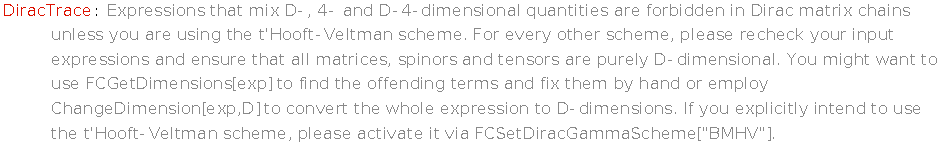
\includegraphics[width=0.6\linewidth]{img/161ti5temvheu.pdf}
\end{figure}

\begin{dmath*}\breakingcomma
\text{\$Aborted}
\end{dmath*}

By default, FeynCalc uses the naive dimensional regularization (NDR)
scheme, where all Dirac matrices are taken to be \(D\)-dimensional.
Therefore, in NDR you may not have mixtures of Dirac matrices living in
\(D\) and \(4\) dimensions. However, such expressions are possible in
the t'Hooft-Veltman-Breitenlohner-Maison (BMHV) scheme.

\begin{Shaded}
\begin{Highlighting}[]
\NormalTok{FCSetDiracGammaScheme}\OperatorTok{[}\StringTok{"BMHV"}\OperatorTok{]}\NormalTok{; }
 
\NormalTok{DiracSimplify}\OperatorTok{[}\NormalTok{GAD}\OperatorTok{[}\SpecialCharTok{\textbackslash{}}\OperatorTok{[}\NormalTok{Mu}\OperatorTok{]]}\NormalTok{ . (GA}\OperatorTok{[}\FunctionTok{p}\OperatorTok{]} \SpecialCharTok{+} \FunctionTok{m}\NormalTok{) . GAD}\OperatorTok{[}\SpecialCharTok{\textbackslash{}}\OperatorTok{[}\NormalTok{Mu}\OperatorTok{]]]}
\end{Highlighting}
\end{Shaded}

\begin{dmath*}\breakingcomma
-D \bar{\gamma }^p+2 \bar{\gamma }^p+D m
\end{dmath*}

\begin{Shaded}
\begin{Highlighting}[]
\NormalTok{FCSetDiracGammaScheme}\OperatorTok{[}\StringTok{"NDR"}\OperatorTok{]}\NormalTok{;}
\end{Highlighting}
\end{Shaded}

The BMHV scheme is a special prescription for handling \(\gamma^5\) in
dimensional regularization. Do not activate this scheme mindlessly just
to get rid of errors from DiracSimplify! If you are doing a calculation
in NDR or a calculation that does not involve \(\gamma^5\), better make
sure that your input expressions are correctly written to be
\(D\)-dimensional objects.

Traces that contain an odd number of \(\gamma^5\) or chirality
projectors cannot be calculated unambiguously in NDR. To avoid
inconsistencies, DiracTrace will refuse to evaluate such traces in NDR.

\begin{Shaded}
\begin{Highlighting}[]
\NormalTok{DiracTrace}\OperatorTok{[}\NormalTok{GAD}\OperatorTok{[}\SpecialCharTok{\textbackslash{}}\OperatorTok{[}\NormalTok{Mu}\OperatorTok{],} \SpecialCharTok{\textbackslash{}}\OperatorTok{[}\NormalTok{Nu}\OperatorTok{],} \SpecialCharTok{\textbackslash{}}\OperatorTok{[}\NormalTok{Rho}\OperatorTok{],} \SpecialCharTok{\textbackslash{}}\OperatorTok{[}\NormalTok{Sigma}\OperatorTok{],} \SpecialCharTok{\textbackslash{}}\OperatorTok{[}\NormalTok{Alpha}\OperatorTok{],} \SpecialCharTok{\textbackslash{}}\OperatorTok{[}\FunctionTok{Beta}\OperatorTok{]]}\NormalTok{ . GA}\OperatorTok{[}\DecValTok{5}\OperatorTok{]]} 
 
\NormalTok{DiracSimplify}\OperatorTok{[}\SpecialCharTok{\%}\OperatorTok{]}
\end{Highlighting}
\end{Shaded}

\begin{dmath*}\breakingcomma
\text{tr}\left(\gamma ^{\mu }.\gamma ^{\nu }.\gamma ^{\rho }.\gamma ^{\sigma }.\gamma ^{\alpha }.\gamma ^{\beta }.\bar{\gamma }^5\right)
\end{dmath*}

\begin{dmath*}\breakingcomma
\text{tr}\left(\gamma ^{\mu }.\gamma ^{\nu }.\gamma ^{\rho }.\gamma ^{\sigma }.\gamma ^{\alpha }.\gamma ^{\beta }.\bar{\gamma }^5\right)
\end{dmath*}

Such traces can be consistently calculated in the BMHV scheme. Our
scheme choice as of course also possible, but those are not implemented
in FeynCalc.

\begin{Shaded}
\begin{Highlighting}[]
\NormalTok{FCSetDiracGammaScheme}\OperatorTok{[}\StringTok{"BMHV"}\OperatorTok{]}\NormalTok{; }
 
\NormalTok{DiracSimplify}\OperatorTok{[}\NormalTok{DiracTrace}\OperatorTok{[}\NormalTok{GAD}\OperatorTok{[}\SpecialCharTok{\textbackslash{}}\OperatorTok{[}\NormalTok{Mu}\OperatorTok{],} \SpecialCharTok{\textbackslash{}}\OperatorTok{[}\NormalTok{Nu}\OperatorTok{],} \SpecialCharTok{\textbackslash{}}\OperatorTok{[}\NormalTok{Rho}\OperatorTok{],} \SpecialCharTok{\textbackslash{}}\OperatorTok{[}\NormalTok{Sigma}\OperatorTok{],} \SpecialCharTok{\textbackslash{}}\OperatorTok{[}\NormalTok{Alpha}\OperatorTok{],} \SpecialCharTok{\textbackslash{}}\OperatorTok{[}\FunctionTok{Beta}\OperatorTok{]]}\NormalTok{ . GA}\OperatorTok{[}\DecValTok{5}\OperatorTok{]]]}
\end{Highlighting}
\end{Shaded}

\begin{dmath*}\breakingcomma
-4 i g^{\alpha \beta } \bar{\epsilon }^{\mu \nu \rho \sigma }-4 i g^{\alpha \mu } \bar{\epsilon }^{\beta \nu \rho \sigma }+4 i g^{\alpha \nu } \bar{\epsilon }^{\beta \mu \rho \sigma }-4 i g^{\alpha \rho } \bar{\epsilon }^{\beta \mu \nu \sigma }+4 i g^{\alpha \sigma } \bar{\epsilon }^{\beta \mu \nu \rho }+4 i g^{\beta \mu } \bar{\epsilon }^{\alpha \nu \rho \sigma }-4 i g^{\beta \nu } \bar{\epsilon }^{\alpha \mu \rho \sigma }+4 i g^{\beta \rho } \bar{\epsilon }^{\alpha \mu \nu \sigma }-4 i g^{\beta \sigma } \bar{\epsilon }^{\alpha \mu \nu \rho }-4 i g^{\mu \nu } \bar{\epsilon }^{\alpha \beta \rho \sigma }+4 i g^{\mu \rho } \bar{\epsilon }^{\alpha \beta \nu \sigma }-4 i g^{\mu \sigma } \bar{\epsilon }^{\alpha \beta \nu \rho }-4 i g^{\nu \rho } \bar{\epsilon }^{\alpha \beta \mu \sigma }+4 i g^{\nu \sigma } \bar{\epsilon }^{\alpha \beta \mu \rho }-4 i g^{\rho \sigma } \bar{\epsilon }^{\alpha \beta \mu \nu }
\end{dmath*}

\begin{Shaded}
\begin{Highlighting}[]
\NormalTok{FCSetDiracGammaScheme}\OperatorTok{[}\StringTok{"NDR"}\OperatorTok{]}\NormalTok{;}
\end{Highlighting}
\end{Shaded}

Keep in mind that the BMHV scheme violates axial Ward identities and
requires special model-dependent counter-terms to restore those.
Therefore, just setting
\texttt{FCSetDiracGammaScheme[\allowbreak{}"BMHV"]} does not magically
resolve all your troubles with \(\gamma^5\) in \(D\)-dimensions. The
proper treatment of \(\gamma^5\) in dimensional regularization is an
intricate issue that cannot be boiled down to a simple and universal
recipe. FeynCalc merely carries out the algebraic operations that you
request, but it is still your task to ensure that what you do makes
sense.

Since FeynCalc 9.3 it is also possible to simplify Dirac matrices with
Cartesian or temporal indices. However, the support of nonrelativistic
calculations is a very new feature, so that things may not work as
smooth as they do for manifestly Lorentz covariant expressions.

\begin{Shaded}
\begin{Highlighting}[]
\NormalTok{CGA}\OperatorTok{[}\FunctionTok{i}\OperatorTok{]}\NormalTok{ . CGA}\OperatorTok{[}\FunctionTok{i}\OperatorTok{]} 
 
\NormalTok{DiracSimplify}\OperatorTok{[}\SpecialCharTok{\%}\OperatorTok{]}
\end{Highlighting}
\end{Shaded}

\begin{dmath*}\breakingcomma
\overline{\gamma }^i.\overline{\gamma }^i
\end{dmath*}

\begin{dmath*}\breakingcomma
-3
\end{dmath*}

\begin{Shaded}
\begin{Highlighting}[]
\NormalTok{CGA}\OperatorTok{[}\FunctionTok{i}\OperatorTok{]}\NormalTok{ . CGS}\OperatorTok{[}\FunctionTok{p}\OperatorTok{]}\NormalTok{ . CGA}\OperatorTok{[}\FunctionTok{j}\OperatorTok{]}\NormalTok{ . CGS}\OperatorTok{[}\FunctionTok{p} \SpecialCharTok{+} \FunctionTok{q}\OperatorTok{]} 
 
\NormalTok{DiracSimplify}\OperatorTok{[}\SpecialCharTok{\%}\OperatorTok{]}
\end{Highlighting}
\end{Shaded}

\begin{dmath*}\breakingcomma
\overline{\gamma }^i.\left(\overline{\gamma }\cdot \overline{p}\right).\overline{\gamma }^j.\left(\overline{\gamma }\cdot \left(\overline{p}+\overline{q}\right)\right)
\end{dmath*}

\begin{dmath*}\breakingcomma
\overline{p}^2 \overline{\gamma }^i.\overline{\gamma }^j-2 \overline{p}^j \overline{\gamma }^i.\left(\overline{\gamma }\cdot \overline{p}\right)+\overline{\gamma }^i.\left(\overline{\gamma }\cdot \overline{p}\right).\overline{\gamma }^j.\left(\overline{\gamma }\cdot \overline{q}\right)
\end{dmath*}

\begin{Shaded}
\begin{Highlighting}[]
\NormalTok{CGA}\OperatorTok{[}\FunctionTok{i}\OperatorTok{]}\NormalTok{ . CGS}\OperatorTok{[}\FunctionTok{p}\OperatorTok{]}\NormalTok{ . CGA}\OperatorTok{[}\FunctionTok{j}\OperatorTok{]}\NormalTok{ . CGS}\OperatorTok{[}\FunctionTok{p} \SpecialCharTok{+} \FunctionTok{q}\OperatorTok{]}\NormalTok{ KD}\OperatorTok{[}\FunctionTok{i}\OperatorTok{,} \FunctionTok{j}\OperatorTok{]} 
 
\NormalTok{DiracSimplify}\OperatorTok{[}\SpecialCharTok{\%}\OperatorTok{]}
\end{Highlighting}
\end{Shaded}

\begin{dmath*}\breakingcomma
\bar{\delta }^{ij} \overline{\gamma }^i.\left(\overline{\gamma }\cdot \overline{p}\right).\overline{\gamma }^j.\left(\overline{\gamma }\cdot \left(\overline{p}+\overline{q}\right)\right)
\end{dmath*}

\begin{dmath*}\breakingcomma
\left(\overline{\gamma }\cdot \overline{p}\right).\left(\overline{\gamma }\cdot \overline{q}\right)-\overline{p}^2
\end{dmath*}

\begin{Shaded}
\begin{Highlighting}[]
\NormalTok{TGA}\OperatorTok{[]}\NormalTok{ . CGA}\OperatorTok{[}\FunctionTok{i}\OperatorTok{]}\NormalTok{ . TGA}\OperatorTok{[]} 
 
\NormalTok{DiracSimplify}\OperatorTok{[}\SpecialCharTok{\%}\OperatorTok{]}
\end{Highlighting}
\end{Shaded}

\begin{dmath*}\breakingcomma
\bar{\gamma }^0.\overline{\gamma }^i.\bar{\gamma }^0
\end{dmath*}

\begin{dmath*}\breakingcomma
-\overline{\gamma }^i
\end{dmath*}

\begin{Shaded}
\begin{Highlighting}[]
\NormalTok{DiracTrace}\OperatorTok{[}\NormalTok{CGAD}\OperatorTok{[}\FunctionTok{i}\OperatorTok{,} \FunctionTok{j}\OperatorTok{,} \FunctionTok{k}\OperatorTok{,} \FunctionTok{l}\OperatorTok{]]} 
 
\NormalTok{DiracSimplify}\OperatorTok{[}\SpecialCharTok{\%}\OperatorTok{]}
\end{Highlighting}
\end{Shaded}

\begin{dmath*}\breakingcomma
\text{tr}\left(\gamma ^i.\gamma ^j.\gamma ^k.\gamma ^l\right)
\end{dmath*}

\begin{dmath*}\breakingcomma
4 \delta ^{il} \delta ^{jk}-4 \delta ^{ik} \delta ^{jl}+4 \delta ^{ij} \delta ^{kl}
\end{dmath*}

For performance reasons \texttt{DiracSimplify} will not canonically
order Dirac matrices and canonicalize Lorentz/Cartesian indices by
default. However, amplitudes involving 4-fermion operators may require
such additional simplifications. In this case they should explicitly
activated by the user. Of course, this will somewhat slow down the
evaluation.

\begin{Shaded}
\begin{Highlighting}[]
\NormalTok{ex }\ExtensionTok{=}\NormalTok{ (Spinor}\OperatorTok{[}\SpecialCharTok{{-}}\NormalTok{Momentum}\OperatorTok{[}\NormalTok{p1}\OperatorTok{,} \FunctionTok{D}\OperatorTok{],}\NormalTok{ mb}\OperatorTok{,} \DecValTok{1}\OperatorTok{]}\NormalTok{ . GAD}\OperatorTok{[}\SpecialCharTok{\textbackslash{}}\OperatorTok{[}\NormalTok{Mu}\OperatorTok{]]}\NormalTok{ . GA}\OperatorTok{[}\DecValTok{7}\OperatorTok{]}\NormalTok{ . GAD}\OperatorTok{[}\SpecialCharTok{\textbackslash{}}\OperatorTok{[}\NormalTok{Nu}\OperatorTok{]]}\NormalTok{ . GAD}\OperatorTok{[}\SpecialCharTok{\textbackslash{}}\OperatorTok{[}\NormalTok{Alpha}\OperatorTok{]]}\NormalTok{ . }
\NormalTok{      GAD}\OperatorTok{[}\SpecialCharTok{\textbackslash{}}\OperatorTok{[}\FunctionTok{Beta}\OperatorTok{]]}\NormalTok{ . GAD}\OperatorTok{[}\SpecialCharTok{\textbackslash{}}\OperatorTok{[}\NormalTok{Delta}\OperatorTok{]]}\NormalTok{ . GA}\OperatorTok{[}\DecValTok{7}\OperatorTok{]}\NormalTok{ . Spinor}\OperatorTok{[}\SpecialCharTok{{-}}\NormalTok{Momentum}\OperatorTok{[}\NormalTok{p4}\OperatorTok{,} \FunctionTok{D}\OperatorTok{],} \DecValTok{0}\OperatorTok{,} \DecValTok{1}\OperatorTok{]}\NormalTok{ Spinor}\OperatorTok{[}\NormalTok{Momentum}\OperatorTok{[}\NormalTok{p3}\OperatorTok{,} \FunctionTok{D}\OperatorTok{],} \DecValTok{0}\OperatorTok{,} 
       \DecValTok{1}\OperatorTok{]}\NormalTok{ . GAD}\OperatorTok{[}\SpecialCharTok{\textbackslash{}}\OperatorTok{[}\NormalTok{Alpha}\OperatorTok{]]}\NormalTok{ . GAD}\OperatorTok{[}\SpecialCharTok{\textbackslash{}}\OperatorTok{[}\FunctionTok{Beta}\OperatorTok{]]}\NormalTok{ . GAD}\OperatorTok{[}\SpecialCharTok{\textbackslash{}}\OperatorTok{[}\NormalTok{Delta}\OperatorTok{]]}\NormalTok{ . GA}\OperatorTok{[}\DecValTok{7}\OperatorTok{]}\NormalTok{ . GAD}\OperatorTok{[}\SpecialCharTok{\textbackslash{}}\OperatorTok{[}\NormalTok{Nu}\OperatorTok{]]}\NormalTok{ . GAD}\OperatorTok{[}\SpecialCharTok{\textbackslash{}}\OperatorTok{[}\NormalTok{Mu}\OperatorTok{]]}\NormalTok{ . }
\NormalTok{      GA}\OperatorTok{[}\DecValTok{7}\OperatorTok{]}\NormalTok{ . Spinor}\OperatorTok{[}\NormalTok{Momentum}\OperatorTok{[}\NormalTok{p2}\OperatorTok{,} \FunctionTok{D}\OperatorTok{],} \DecValTok{0}\OperatorTok{,} \DecValTok{1}\OperatorTok{]}\NormalTok{) }
 
\NormalTok{DiracSimplify}\OperatorTok{[}\NormalTok{ex}\OperatorTok{]}
\end{Highlighting}
\end{Shaded}

\begin{dmath*}\breakingcomma
(\varphi (\text{p3})).\gamma ^{\alpha }.\gamma ^{\beta }.\gamma ^{\delta }.\bar{\gamma }^7.\gamma ^{\nu }.\gamma ^{\mu }.\bar{\gamma }^7.(\varphi (\text{p2})) (\varphi (-\text{p1},\text{mb})).\gamma ^{\mu }.\bar{\gamma }^7.\gamma ^{\nu }.\gamma ^{\alpha }.\gamma ^{\beta }.\gamma ^{\delta }.\bar{\gamma }^7.(\varphi (-\text{p4}))
\end{dmath*}

\begin{dmath*}\breakingcomma
(\varphi (\text{p3})).\gamma ^{\alpha }.\gamma ^{\beta }.\gamma ^{\delta }.\gamma ^{\nu }.\gamma ^{\mu }.\bar{\gamma }^7.(\varphi (\text{p2})) (\varphi (-\text{p1},\text{mb})).\gamma ^{\mu }.\gamma ^{\nu }.\gamma ^{\alpha }.\gamma ^{\beta }.\gamma ^{\delta }.\bar{\gamma }^7.(\varphi (-\text{p4}))
\end{dmath*}

\begin{Shaded}
\begin{Highlighting}[]
\NormalTok{DiracSimplify}\OperatorTok{[}\NormalTok{ex}\OperatorTok{,}\NormalTok{ DiracOrder }\OtherTok{{-}\textgreater{}} \ConstantTok{True}\OperatorTok{,}\NormalTok{ LorentzIndexNames }\OtherTok{{-}\textgreater{}} \OperatorTok{\{}\NormalTok{i1}\OperatorTok{,}\NormalTok{ i2}\OperatorTok{,}\NormalTok{ i3}\OperatorTok{,}\NormalTok{ i4}\OperatorTok{,}\NormalTok{ i5}\OperatorTok{\}]}
\end{Highlighting}
\end{Shaded}

\begin{dmath*}\breakingcomma
-24 D^2 (\varphi (\text{p3})).\gamma ^{\text{i1}}.\bar{\gamma }^7.(\varphi (\text{p2})) (\varphi (-\text{p1},\text{mb})).\gamma ^{\text{i1}}.\bar{\gamma }^7.(\varphi (-\text{p4}))+14 D (\varphi (\text{p3})).\gamma ^{\text{i1}}.\gamma ^{\text{i2}}.\gamma ^{\text{i3}}.\bar{\gamma }^7.(\varphi (\text{p2})) (\varphi (-\text{p1},\text{mb})).\gamma ^{\text{i1}}.\gamma ^{\text{i2}}.\gamma ^{\text{i3}}.\bar{\gamma }^7.(\varphi (-\text{p4}))+112 D (\varphi (\text{p3})).\gamma ^{\text{i1}}.\bar{\gamma }^7.(\varphi (\text{p2})) (\varphi (-\text{p1},\text{mb})).\gamma ^{\text{i1}}.\bar{\gamma }^7.(\varphi (-\text{p4}))-(\varphi (\text{p3})).\gamma ^{\text{i1}}.\gamma ^{\text{i2}}.\gamma ^{\text{i3}}.\gamma ^{\text{i4}}.\gamma ^{\text{i5}}.\bar{\gamma }^7.(\varphi (\text{p2})) (\varphi (-\text{p1},\text{mb})).\gamma ^{\text{i1}}.\gamma ^{\text{i2}}.\gamma ^{\text{i3}}.\gamma ^{\text{i4}}.\gamma ^{\text{i5}}.\bar{\gamma }^7.(\varphi (-\text{p4}))-36 (\varphi (\text{p3})).\gamma ^{\text{i1}}.\gamma ^{\text{i2}}.\gamma ^{\text{i3}}.\bar{\gamma }^7.(\varphi (\text{p2})) (\varphi (-\text{p1},\text{mb})).\gamma ^{\text{i1}}.\gamma ^{\text{i2}}.\gamma ^{\text{i3}}.\bar{\gamma }^7.(\varphi (-\text{p4}))-64 (\varphi (\text{p3})).\gamma ^{\text{i1}}.\bar{\gamma }^7.(\varphi (\text{p2})) (\varphi (-\text{p1},\text{mb})).\gamma ^{\text{i1}}.\bar{\gamma }^7.(\varphi (-\text{p4}))
\end{dmath*}

\texttt{DiracSimplify} automatically evaluates suitable spinor products
with equal momenta, e.g.

\begin{Shaded}
\begin{Highlighting}[]
\NormalTok{ex }\ExtensionTok{=}\NormalTok{ SpinorUBar}\OperatorTok{[}\FunctionTok{p}\OperatorTok{,} \FunctionTok{m}\OperatorTok{]}\NormalTok{ . SpinorU}\OperatorTok{[}\FunctionTok{p}\OperatorTok{,} \FunctionTok{m}\OperatorTok{]} 
 
\NormalTok{DiracSimplify}\OperatorTok{[}\NormalTok{ex}\OperatorTok{]}
\end{Highlighting}
\end{Shaded}

\begin{dmath*}\breakingcomma
\bar{u}(p,m).u(p,m)
\end{dmath*}

\begin{dmath*}\breakingcomma
2 m
\end{dmath*}

This behavior can be turned off by setting the option
\texttt{SpinorChainEvaluate} to \texttt{False}

\begin{Shaded}
\begin{Highlighting}[]
\NormalTok{DiracSimplify}\OperatorTok{[}\NormalTok{ex}\OperatorTok{,}\NormalTok{ SpinorChainEvaluate }\OtherTok{{-}\textgreater{}} \ConstantTok{False}\OperatorTok{]}
\end{Highlighting}
\end{Shaded}

\begin{dmath*}\breakingcomma
\left(\varphi (\overline{p},m)\right).\left(\varphi (\overline{p},m)\right)
\end{dmath*}
\end{document}
